\documentclass[11pt]{article}
\usepackage[margin=1in]{geometry}
\usepackage{amsmath,amssymb,amsthm}
\usepackage{algorithm}
\usepackage{algpseudocode}
\usepackage{booktabs}
\usepackage{hyperref}
\usepackage{tikz}
\usepackage{xcolor}
\usetikzlibrary{arrows.meta,positioning,fit,backgrounds,shapes.geometric,calc}

\newtheorem{theorem}{Theorem}
\newtheorem{proposition}{Proposition}
\newtheorem{lemma}{Lemma}
\newtheorem{definition}{Definition}
\newtheorem{example}{Example}
\newtheorem{corollary}{Corollary}
\newtheorem{remark}{Remark}

\newcommand{\lo}{\underline}
\newcommand{\hi}{\overline}
\newcommand{\indep}{\perp\!\!\!\perp}
\newcommand{\DSE}{\mathcal{D}_{\mathrm{SE}}}
\newcommand{\DLCN}{\mathcal{D}_{\mathrm{LCN}}}
\newcommand{\ch}{\mathrm{ch}}
\newcommand{\pa}{\mathrm{pa}}
\newcommand{\atoms}{\mathrm{atoms}}

\title{When are the strong-extension engines exact?\\
\large A formal analysis of the credal-network boundary case, and the exact
characterization of exactness for Credal~VE and Interval~BP}
\author{IBM Research}
\date{}

\begin{document}
\maketitle

\begin{abstract}
The credal-network engines that bound the \emph{strong extension} $\DSE$ --- Credal~VE (exact over
$\DSE$) and Interval~BP (outer over $\DSE$; exact on trees) --- are known to be exact with respect to
the LCN's true distribution set $\DLCN$ on a singly-connected LCN \emph{with no cross-family
sentence}, where ``cross-family'' is judged by whether a sentence's atom scope fits inside a single
family scope. This note shows that atom-scope cross-family membership is \emph{not} the condition that
actually governs exactness. We exhibit a shipped singly-connected tree,
\texttt{benchmarks/tree\_small/tree\_n5\_1.lcn}, on which every sentence is atom-scope family-local yet
Credal~VE and Interval~BP are strictly loose ($P(x_2)=[0,0.8012]$ against the exact $[0.010,0.4395]$).
We identify the true governing property --- a sentence is \emph{family-realizable} iff the quantity it
bounds is a function of one family's \emph{conditional} $P(\ch_v\mid\pa_v)$ alone, rather than a
function that also depends on the parents' marginal $P(\pa_v)$ --- and prove the sharp
characterization: with the \texttt{"linear"} local sets, $\DSE=\DLCN$ (equivalently Credal~VE, and
Interval~BP on a tree, is exact for every atom) \emph{if and only if} the primal graph is singly
connected and every sentence is family-realizable. The familiar ``no cross-family sentence'' condition
is exactly the atom-scope-visible half of family-realizability; the invisible half has two forms, both
atom-scope family-local: (a)~a Type-1 formula mentioning a non-root child (a bare marginal $P(x)$ or a
child--parent joint $P(x\wedge\text{parent})$), and (b)~a Type-2 sentence whose condition $\psi$ is a
\emph{formula} satisfied by two or more parent configurations --- the \emph{collider} case
$P(x_2\mid x_1\oplus x_3)$, which binds through the co-parents' joint (their LMC independence).
Crucially, this looseness is a property of the strong extension, not the solver: we confirm that
neither the certified global SCIP solver nor the LMC-tightening scheme~D1 recovers the bound, because
the coupling cannot be represented as a product of per-parent-config conditional credal sets; the
exact route is scheme~D2 (merge) or the junction-tree engine \texttt{CredalJT} (D5). We give the full
\texttt{tree\_n5\_1} derivation, minimal witnesses (including the solver-invariant collider), a remark
that a non-realizable sentence can even mask an inconsistency, a complete case catalogue over
(sentence shape) $\times$ (node role), and the engine-specific consequences and fixes.
\end{abstract}

\tableofcontents

\section{Setup}\label{sec:setup}

We recap only what we need; see \texttt{docs/properties.tex} and \texttt{docs/cve\_exactness.tex} for
the full framework.

An LCN over binary atoms $\mathbf V$ has a set of \emph{sentences} (Type-1 $\ell\le P(\varphi)\le u$
or Type-2 $\ell\le P(\varphi\mid\psi)\le u$) and the Local Markov Condition (LMC) of its primal graph;
together they define the \emph{LCN distribution set} $\DLCN\subseteq\Delta(2^{\mathbf V})$ of joints
satisfying every sentence and every LMC equality. The chain-graph factorization splits the joint into
\emph{families} $P(\ch_v\mid\pa_v)$, one per node $v$ of the simplified structure graph; the family's
\emph{scope} is $\ch_v\cup\pa_v$. Root families have $\pa_v=\varnothing$, so their factor is the plain
marginal $P(\ch_v)$.

For each family the \texttt{cn/} pipeline (\texttt{lcn/inference/marginal/cn/local\_credal\_sets.py},
\texttt{method="linear"}) computes a \emph{local credal set} $K_v$: the set of conditional tables
$P(\ch_v\mid\pa_v)$ attainable by \emph{some} joint that satisfies the sentences whose atom scope lies
inside the family scope. Operationally it is a linear-fractional program
$P(\ch_v,\pa_v)/P(\pa_v)$ solved by the Charnes--Cooper transformation, in which \emph{the parents'
distribution $P(\pa_v)$ is a free variable} --- the program returns the range of the conditional, not
of any marginal. The engines then bound the \emph{strong extension}
\begin{equation}\label{eq:se}
  \DSE=\Bigl\{\textstyle\prod_v P_v \;:\; P_v\in K_v \text{ chosen independently per parent-config}\Bigr\},
\end{equation}
and, because a chain-graph product satisfies every LMC assertion,
\begin{equation}\label{eq:incl}
  \DLCN\;\subseteq\;\DSE .
\end{equation}
Credal~VE returns \emph{exactly} the strong-extension interval $[\lo q_{\mathrm{SE}},\hi
q_{\mathrm{SE}}]$ (\texttt{docs/cve\_exactness.tex}); Interval~BP is an outer bound over $\DSE$ that is
exact on a tree factor graph (\texttt{docs/ibp\_exactness.tex}). Both consume the same enumerated
vertices of the $K_v$, so both are exact with respect to $\DLCN$ for a queried atom \emph{iff}
$\DSE=\DLCN$ there. This note characterizes exactly when that holds.

\section{Family-realizable sentences}\label{sec:realizable}

The key is which sentences a single family's local set can \emph{enforce}. A family's degrees of
freedom are the conditional probabilities $P(\ch_v{=}c\mid\pa_v{=}p)$; the parents' marginal
$P(\pa_v)$ is not one of them (it is fixed elsewhere in the network, and free during the local solve).

\begin{definition}[Family-realizable sentence]\label{def:realizable}
A sentence $s$ is \emph{family-realizable} in family $v$ if the probability it bounds is a function of
the conditional table $P(\ch_v\mid\pa_v)$ \emph{alone} --- i.e.\ its value is unchanged by varying the
parents' distribution $P(\pa_v)$. Concretely this holds iff $s$ is one of:
\begin{itemize}
  \item a Type-1 sentence $P(\varphi)$ on a \emph{root} family ($\pa_v=\varnothing$, so $P(\varphi)$
    \emph{is} a function of $P(\ch_v)$); or
  \item a Type-2 sentence $P(\varphi\mid\psi)$ with $\atoms(\varphi)\subseteq\ch_v$ where the
    condition $\psi$ pins a \emph{single, full} parent-configuration --- i.e.\ exactly one assignment
    of $\pa_v$ satisfies $\psi$. Then $P(\varphi\mid\psi)$ is a single row of the conditional table,
    independent of $P(\pa_v)$.
\end{itemize}
A sentence is \emph{non-realizable} otherwise. Note the Type-2 clause is subtler than
``$\atoms(\psi)\subseteq\pa_v$'': if $\psi$ is a \emph{formula} satisfied by two or more parent
configurations (e.g.\ $x_1\oplus x_3$), then
$P(\varphi\mid\psi)=\sum_{c\models\psi}P(\varphi,c)\big/\sum_{c\models\psi}P(c)$ is a
$P(\pa_v)$-weighted mixture of conditional rows --- a function of the parents' \emph{joint}
distribution, hence non-realizable even though $\atoms(\psi)\subseteq\pa_v$
(Remark~\ref{rem:scope}, Example~\ref{ex:collider}). An LCN is \emph{fully realizable} if every
sentence is family-realizable in some family.
\end{definition}

\begin{remark}[Atom scope is not enough]\label{rem:scope}
Family-realizability is strictly stronger than the atom-scope ``fits in a family'' test. A Type-1
sentence $P(\varphi)$ whose formula $\varphi$ mentions a \emph{non-root} child $x$ has atoms that may
well sit inside a family scope, yet it bounds a \emph{marginal or joint} of $p$, not a conditional.
Since for a non-root node $P(\varphi)=\sum_{\pa}P(\varphi\mid\pa)\,P(\pa)$ depends on the parents'
marginal, it is not a function of any one family's conditional and is therefore non-realizable. Two
canonical offenders, both atom-scope family-local:
\begin{itemize}
  \item a \textbf{bare marginal on a non-root child}, $P(x)$ with $\pa_x\neq\varnothing$ (atoms
    $\{x\}\subseteq$ every family containing $x$);
  \item a \textbf{child--parent joint}, $P(x\wedge y)$ with $y=\pa_x$ (atoms $\{x,y\}=$ the family
    scope of $x\mid y$), which equals $P(x\mid y)\,P(y)$ and again couples the conditional to $P(y)$;
  \item a \textbf{multi-configuration-$\psi$ Type-2 sentence at a collider}, $P(\varphi\mid\psi)$
    where $\psi$ is a formula satisfied by $\ge2$ parent configurations (e.g.\
    $P(x_2\mid x_1\oplus x_3)$ with co-parents $x_1,x_3$). Its value mixes conditional rows weighted
    by $P(\pa_v)$; equivalently it binds through the co-parents' joint, which for a collider is
    governed by the co-parent LMC assertion $x_1\indep x_3$ --- a \emph{joint} constraint the
    per-parent-config credal set cannot carry.
\end{itemize}
\emph{This is not a solver, tightening-scheme, or enumeration artifact.} We verified that neither the
global SCIP backend nor scheme~D1 (\texttt{"linear-tight"}, which \emph{does} add the co-parent LMC
bilinear equality to the family solve) recovers the bound: the offending family's per-parent-config
extreme points are genuinely the full box (each individual row is unconstrained; only a
$P(\pa_v)$-weighted mixture is), so any representation of the family as a product of independent
per-config conditional credal sets loses the coupling. The bound is recoverable only by keeping the
coupled atoms in one joint block --- scheme~D2 (merge the family with its parents) or the exact
junction-tree engine \texttt{CredalJT} (D5), which is precisely why D5 stays exact here while
Credal~VE / Interval~BP cannot.
\end{remark}

\section{The exactness characterization}\label{sec:theorem}

\begin{theorem}[Exactness of the strong-extension engines]\label{thm:main}
Let $\mathcal L$ be a chain-graph LCN whose local credal sets are built by the \texttt{"linear"}
method. Then $\DSE=\DLCN$ --- equivalently, Credal~VE (and Interval~BP on the tree factor graph) is
exact with respect to $\DLCN$ for every atom --- \emph{if and only if}
\begin{enumerate}
  \item[\textup{(i)}] the primal graph is singly connected, and
  \item[\textup{(ii)}] every sentence is family-realizable (Definition~\ref{def:realizable}).
\end{enumerate}
\end{theorem}

\begin{proof}
\emph{Sufficiency.} Assume (i) and (ii). Fix a family $v$. Because every sentence constraining atoms
inside $\ch_v\cup\pa_v$ is family-realizable, it bounds a functional of the conditional
$P(\ch_v\mid\pa_v)$ only; hence $K_v$, the range of that conditional over joints meeting these
sentences, is precisely the projection of $\DLCN$ onto the family's conditional (no Gap~A on the
imposed conditional: nothing that constrains the conditional was omitted, and nothing imposed
constrains anything but the conditional). Now take any product $\prod_v P_v$ with $P_v\in K_v$. Being a
chain-graph product it satisfies every LMC assertion by construction; and every sentence, being a
function of a single family's conditional $P_v$ with $P_v\in K_v$, is satisfied. Therefore
$\prod_v P_v\in\DLCN$, giving $\DSE\subseteq\DLCN$; with \eqref{eq:incl}, $\DSE=\DLCN$. (Single
connectedness guarantees the primal graph moralizes to a chain graph whose families are exactly these
factors, so the product form is the general element of $\DLCN$.)

\emph{Necessity.} Suppose (ii) fails: some sentence $s$ is non-realizable in its family $v$, i.e.\ the
quantity $g$ it bounds is a genuine function $g\bigl(P(\ch_v\mid\pa_v),P(\pa_v)\bigr)$ that depends on
$P(\pa_v)$. The local set $K_v$ is built with $P(\pa_v)$ free, so it retains every conditional table
$P(\ch_v\mid\pa_v)$ that is consistent with $s$ under \emph{some} choice of $P(\pa_v)$ --- including
tables that violate $s$ under the parents' \emph{actual} network marginal. In the free product
\eqref{eq:se} the vertex chosen for $v$ and the marginal $P(\pa_v)$ induced by the other families are
selected independently, so $\DSE$ contains a product joint on which $g$ falls outside $[\ell_s,u_s]$;
that joint is not in $\DLCN$. Hence $\DSE\supsetneq\DLCN$, and the affected marginal's
strong-extension range strictly contains its $\DLCN$ range, so the engines are strictly loose there.
The failure of (i) (a loop in the primal graph) makes $\DSE\supsetneq\DLCN$ for the standard reason
(the free product cannot reproduce the correlation carried by a second path); see
\texttt{docs/properties.tex}. Constructive witnesses for the (ii) direction are
Examples~\ref{ex:2node} (a non-root marginal) and~\ref{ex:collider} (a multi-configuration collider
condition, whose looseness is invariant to solver and to scheme~D1).
\end{proof}

\begin{corollary}[Refinement of ``no cross-family sentence'']\label{cor:refine}
The condition ``singly connected and no cross-family sentence'' used in the companion notes is exactly
the atom-scope-visible special case of Theorem~\ref{thm:main}: an atom-scope cross-family sentence is
always non-realizable, but so is a Type-1 formula mentioning a non-root child even though its atoms are
family-local. Family-realizability is the sharp condition; ``no cross-family sentence'' is sufficient
for the sentences it can see and silent about the rest.
\end{corollary}

\begin{remark}[A non-realizable sentence can mask an inconsistency]\label{rem:mask}
Because a non-realizable sentence is dropped from every family's enforceable set, $\DSE$ can be
non-empty even when $\DLCN=\varnothing$. Adding \texttt{M1: $P(x_1)\le0.25$} to the chain of
Example~\ref{ex:2node} makes $\DLCN$ empty (the transitions force $P(x_1)\ge0.4$), which the exact
engine \texttt{CredalJT} flags as degenerate ($[0,1]$ everywhere), yet Credal~VE returns the
non-empty strong-extension bound $P(x_0)=[0.3,0.5]$. The strong-extension engines therefore cannot be
used to certify (in)consistency in the presence of non-realizable sentences.
\end{remark}

\section{Worked example: \texttt{tree\_n5\_1.lcn}}\label{sec:tree}

The instance (a saved 5-atom tree) is
\begin{center}\small
\begin{tabular}{ll}
\texttt{s0}: $0.159\le P(\lnot x_3)\le0.759$ & \texttt{s4}: $0.01\le P(x_0\mid\lnot x_2)\le0.323$\\
\texttt{s1}: $0.351\le P(x_4\mid\lnot x_3)\le0.951$ & \texttt{s5}: $0.01\le P(x_2)\le0.4395$\\
\texttt{s2}: $0.639\le P(\lnot x_2\mid x_3)\le1.0$ & \texttt{s6}: $0.01\le P(x_3)\le0.533$\\
\texttt{s3}: $0.317\le P(\lnot x_1\mid x_4)\le0.917$ &
\end{tabular}
\end{center}
with primal tree $x_3\!\to\!x_2\!\to\!x_0$ and $x_3\!\to\!x_4\!\to\!x_1$ (Figure~\ref{fig:tree},
left). Interval~BP runs on the \emph{bipartite factor graph} that the \texttt{cn/} pipeline builds
from the chain-graph families --- one factor node per family, connected to the variable nodes in its
scope (Figure~\ref{fig:tree}, right); the offending factor $f_2=P(x_2\mid x_3)$, which carries the
non-realizable marginal \texttt{s5}, is highlighted.

\begin{figure}[ht]
\centering
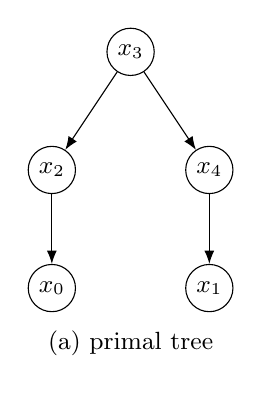
\begin{tikzpicture}[
    >=Latex,
    var/.style={circle,draw,minimum size=6mm,inner sep=0pt,font=\small},
    every node/.style={font=\small}]
  % ---- left: primal directed tree ----
  \begin{scope}
    \node[var] (x3) at (1.0,3.0) {$x_3$};
    \node[var] (x2) at (0.0,1.5) {$x_2$};
    \node[var] (x4) at (2.0,1.5) {$x_4$};
    \node[var] (x0) at (0.0,0.0) {$x_0$};
    \node[var] (x1) at (2.0,0.0) {$x_1$};
    \draw[->] (x3) -- (x2);
    \draw[->] (x3) -- (x4);
    \draw[->] (x2) -- (x0);
    \draw[->] (x4) -- (x1);
    \node[font=\small] at (1.0,-0.7) {(a) primal tree};
  \end{scope}
\end{tikzpicture}
\hspace{1.2cm}
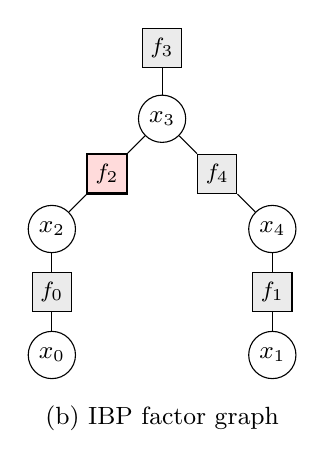
\begin{tikzpicture}[
    >=Latex,
    var/.style={circle,draw,minimum size=6mm,inner sep=0pt,font=\small},
    fac/.style={rectangle,draw,fill=black!8,minimum size=5mm,inner sep=1pt,font=\footnotesize},
    bad/.style={rectangle,draw,fill=red!14,thick,minimum size=5mm,inner sep=1pt,font=\footnotesize},
    every node/.style={font=\small}]
  % ---- right: bipartite factor graph IBP uses ----
  % variable nodes (circles) and factor nodes (squares)
  \node[var] (x3) at (2.0,3.4) {$x_3$};
  \node[fac] (f3) at (2.0,4.3) {$f_3$};              % P(x3)  root prior
  \node[var] (x2) at (0.6,2.0) {$x_2$};
  \node[var] (x4) at (3.4,2.0) {$x_4$};
  \node[bad] (f2) at (1.3,2.7) {$f_2$};              % P(x2|x3)  <-- non-realizable
  \node[fac] (f4) at (2.7,2.7) {$f_4$};              % P(x4|x3)
  \node[var] (x0) at (0.6,0.4) {$x_0$};
  \node[var] (x1) at (3.4,0.4) {$x_1$};
  \node[fac] (f0) at (0.6,1.2) {$f_0$};              % P(x0|x2)
  \node[fac] (f1) at (3.4,1.2) {$f_1$};              % P(x1|x4)
  \draw (f3) -- (x3);
  \draw (f2) -- (x3);   \draw (f2) -- (x2);
  \draw (f4) -- (x3);   \draw (f4) -- (x4);
  \draw (f0) -- (x2);   \draw (f0) -- (x0);
  \draw (f1) -- (x4);   \draw (f1) -- (x1);
  \node[font=\small] at (2.0,-0.4) {(b) IBP factor graph};
\end{tikzpicture}
\caption{\texttt{tree\_n5\_1.lcn}. (a) The primal directed tree. (b) The bipartite factor graph
Interval~BP propagates over: circles are variable (atom) nodes, squares are factor nodes, one per
chain-graph family --- $f_3{=}P(x_3)$ (root prior), $f_2{=}P(x_2\mid x_3)$, $f_4{=}P(x_4\mid x_3)$,
$f_0{=}P(x_0\mid x_2)$, $f_1{=}P(x_1\mid x_4)$ --- each joined to the variables in its scope. The
factor graph is a tree, so a correct interval BP would be exact over $\DSE$; the looseness comes
entirely from factor $f_2$ (shaded), whose non-realizable marginal \texttt{s5}$:P(x_2)\le0.4395$
cannot be enforced locally, so the composed $P(x_2)$ escapes to $[0,0.8012]$ and inflates $x_0$
downstream through $f_0$.}\label{fig:tree}
\end{figure}

The five families and the
realizability of their attached sentences:
\begin{center}\small
\begin{tabular}{llll}
\toprule
family & role & attached sentences & realizable? \\
\midrule
$P(x_3)$        & root      & \texttt{s0},\texttt{s6} (marginals on root $x_3$) & yes \\
$P(x_4\mid x_3)$ & non-root & \texttt{s1} (Type-2 $x_4\mid x_3$) & yes \\
$P(x_1\mid x_4)$ & non-root & \texttt{s3} (Type-2 $x_1\mid x_4$) & yes \\
$P(x_0\mid x_2)$ & non-root & \texttt{s4} (Type-2 $x_0\mid x_2$) & yes \\
$P(x_2\mid x_3)$ & non-root & \texttt{s2} (Type-2), \;\textbf{\texttt{s5}: $P(x_2)$} & \textbf{no (\texttt{s5})} \\
\bottomrule
\end{tabular}
\end{center}
Exactly one sentence is non-realizable: \texttt{s5}, a marginal on the \emph{non-root} child $x_2$.
By Theorem~\ref{thm:main} the instance fails condition (ii), so the strong-extension engines are
loose, and the looseness is localized to the family carrying the non-realizable sentence and its
descendants.

\paragraph{The witness for $x_2$.} The local set for $P(x_2\mid x_3)$ enforces \texttt{s2} (a
conditional) but not \texttt{s5} (the marginal). Composing its extreme points with those of $P(x_3)$
--- the free product of \eqref{eq:se} --- the reachable marginal
$P(x_2{=}1)=\sum_{x_3}P(x_2{=}1\mid x_3)\,P(x_3)$ ranges over $[0,0.8012]$, grossly exceeding
\texttt{s5}'s cap $0.4395$. The exact engines respect \texttt{s5}: \texttt{CredalJT} and ARIEL both
return $P(x_2)=[0.010,0.4395]$, hitting the sentence bound. Credal~VE and Interval~BP return exactly
the strong-extension interval $[0.000,0.8012]$.

\paragraph{Downstream propagation to $x_0$.} $x_0$'s family $P(x_0\mid x_2)$ carries only the Type-2
\texttt{s4} on the $x_2{=}0$ branch, leaving $P(x_0\mid x_2{=}1)$ vacuous. Since
$P(x_0)=P(x_0\mid x_2{=}0)P(x_2{=}0)+P(x_0\mid x_2{=}1)P(x_2{=}1)$, the inflated $P(x_2)$ range
combines with the free $x_2{=}1$ row and lifts $x_0$ from the exact $[0.0056,0.6206]$ to the
strong-extension $[0.002,0.8654]$. The other three atoms are exact:

\begin{center}\small
\begin{tabular}{lccl}
\toprule
atom & Credal~VE / Interval~BP ($\DSE$) & \texttt{CredalJT} / ARIEL (exact) & verdict \\
\midrule
$x_0$ & $[0.0020,0.8654]$ & $[0.0056,0.6206]$ & \textbf{loose} \\
$x_1$ & $[0.0135,0.9480]$ & $[0.0135,0.9480]$ & exact \\
$x_2$ & $[0.0000,0.8012]$ & $[0.0100,0.4395]$ & \textbf{loose} \\
$x_3$ & $[0.2408,0.5328]$ & $[0.2408,0.5328]$ & exact \\
$x_4$ & $[0.1639,0.9771]$ & $[0.1639,0.9771]$ & exact \\
\bottomrule
\end{tabular}
\end{center}
$x_1,x_3,x_4$ are exact because their families carry only realizable sentences (root marginals on
$x_3$; Type-2 conditionals for $x_4\mid x_3$ and $x_1\mid x_4$), matching Theorem~\ref{thm:main}: the
looseness is confined to the non-realizable family $\{x_2\mid x_3\}$ and its descendant $x_0$.

\section{Minimal witnesses}\label{sec:witnesses}

\begin{example}[Marginal on a non-root child]\label{ex:2node}
The two-atom chain $x_0\!\to\!x_1$:
\begin{center}\small
\texttt{P0}: $0.3\le P(x_0)\le0.5$;\quad
\texttt{T0}: $0.2\le P(x_1\mid x_0)\le0.4$;\quad
\texttt{T1}: $0.6\le P(x_1\mid\lnot x_0)\le0.8$;\quad
\texttt{M1}: $0.45\le P(x_1)\le0.55$.
\end{center}
\texttt{M1} is a marginal on the non-root child $x_1$: non-realizable. Credal~VE returns
$P(x_1)=[0.40,0.68]$ (ignoring \texttt{M1}, which its family $P(x_1\mid x_0)$ cannot impose), while the
exact bound is $[0.45,0.55]$; $x_0$ stays exact $[0.30,0.50]$. Removing \texttt{M1} restores exactness
on both atoms. This is the smallest instance exhibiting the boundary.
\end{example}

\begin{example}[Child--parent joint]\label{ex:joint}
With $x_2$ a root and $x_0$ its child:
\begin{center}\small
\texttt{P2}: $0.3\le P(x_2)\le0.6$;\quad
\texttt{T0}: $0.2\le P(x_0\mid x_2)\le0.5$;\quad
\texttt{T1}: $0.1\le P(x_0\mid\lnot x_2)\le0.3$;\quad
\texttt{J}: $0.05\le P(x_0\wedge x_2)\le0.15$.
\end{center}
\texttt{J} has atoms $\{x_0,x_2\}$ --- the entire scope of family $x_0\mid x_2$ --- so it is atom-scope
family-local, yet it bounds $P(x_0\wedge x_2)=P(x_0\mid x_2)\,P(x_2)$, coupling the conditional to
$P(x_2)$: non-realizable. Credal~VE returns $P(x_0)=[0.13,0.42]$ against the exact $[0.13,0.36]$; $x_2$
stays exact $[0.30,0.60]$. This shows the offender need not be a bare marginal, and confirms the atom-scope test cannot detect the case (Remark~\ref{rem:scope}).
\end{example}

\begin{example}[Collider with a multi-configuration condition]\label{ex:collider}
A single collider $x_0\to x_2\leftarrow x_1$ with two roots and one Type-2 sentence whose condition
spans both parents:
\begin{center}\small
\texttt{P0}: $0.3\le P(x_0)\le0.5$;\quad
\texttt{P1}: $0.4\le P(x_1)\le0.6$;\quad
\texttt{C}: $0.2\le P(x_2\mid x_0\oplus x_1)\le0.5$.
\end{center}
Here $\atoms(\psi)=\{x_0,x_1\}\subseteq\pa_{x_2}$, so \texttt{C} passes the naive Type-2 test, but
$\psi=x_0\oplus x_1$ is satisfied by \emph{two} parent configurations, so \texttt{C} is non-realizable
(Definition~\ref{def:realizable}). The exact bound (\texttt{ExactInference} with the global SCIP
solver, both endpoints certified at gap $0$; \texttt{CredalJT} agrees) is
$P(x_2)=[0.092,0.77]$, $P(x_0)=[0.30,0.50]$, $P(x_1)=[0.40,0.60]$. Credal~VE and Interval~BP return
$P(x_2)=[0,1]$ --- fully vacuous --- because the $x_2$ family's per-parent-config extreme points are
each the full box $[0,1]$ (no single row is constrained; only the $\{x_0\!\neq\!x_1\}$ mixture is), so
no product of per-config conditional sets can reproduce the bound. \emph{Neither} the global solver
\emph{nor} scheme~D1 (which adds the co-parent LMC equality $x_0\indep x_1$ to the family solve)
changes this: on the D1 credal network, \texttt{CredalJT} is exact ($[0.092,0.77]$) yet Credal~VE is
still $[0,1]$, isolating the loss to the per-parent-config \emph{representation}, not the solve. The
bound returns only by fusing $\{x_0,x_1,x_2\}$ into one joint block (D2 merge) or via the joint NLP of
\texttt{CredalJT} (D5). This is the witness underlying the loose atom in
\texttt{benchmarks/polytree\_small\_fr/polytree\_fr\_n5\_6.lcn}.
\end{example}

\section{The exactness catalogue}\label{sec:catalogue}

Table~\ref{tab:cat} enumerates the cases; ``realizable?'' is by Definition~\ref{def:realizable} and the
verdict follows from Theorem~\ref{thm:main} (assuming, for the sentence-shape rows, an otherwise
singly-connected, fully-realizable instance so the row's sentence is the only variable).

\begin{table}[ht]\centering\small
\caption{When the strong-extension engines (Credal~VE; Interval~BP on a tree) are exact w.r.t.\
$\DLCN$.}\label{tab:cat}
\begin{tabular}{@{}lccl@{}}
\toprule
Sentence shape / structural feature & realizable? & $\DSE{=}\DLCN$? & engine verdict \\
\midrule
Type-2 $P(\varphi(\ch)\mid\psi)$, $\psi$ pins a \emph{single} parent-config & yes & yes & \textbf{exact} \\
Type-1 $P(\varphi)$ on a \emph{root} family & yes & yes & \textbf{exact} \\
Type-2 $P(\varphi\mid\psi)$, $\psi$ a \emph{multi-config} formula (collider) & \textbf{no} & no & loose (Gap~B) \\
Type-1 $P(\varphi)$ mentioning a \emph{non-root} child & \textbf{no} & no & loose (Gap~B) \\
Type-1 child--parent joint $P(x\wedge\pa_x)$ & \textbf{no} & no & loose (Gap~B) \\
atom-scope cross-family sentence (e.g.\ \texttt{d4\_biting}) & \textbf{no} & no & loose (Gap~B) \\
loopy primal graph (any sentences) & --- & no & loose \\
\bottomrule
\end{tabular}
\end{table}

\noindent For every ``loose (Gap~B)'' row the looseness is a property of the strong extension itself,
\emph{not} of the solver or of scheme~D1: we verified (Example~\ref{ex:collider}) that the certified
global SCIP solver and \texttt{"linear-tight"} both leave the affected marginal loose, because the
coupling is unrepresentable as a product of per-parent-config conditional credal sets. The exact route
for these rows is scheme~D2 (merge the coupled atoms into one joint block) or the junction-tree engine
\texttt{CredalJT} (D5) / \texttt{ExactInference} (global).

\begin{corollary}[Sufficient clean regimes]\label{cor:clean}
A Markov chain, rooted tree, or polytree whose sentences are all root marginals and
conditional-on-parent Type-2 sentences is fully realizable and singly connected; by
Theorem~\ref{thm:main} Credal~VE and Interval~BP are exact on it for every atom. This is the regime the
benchmark generator now targets: \texttt{lcn/benchmarks/generator.py} emits its extra marginal
sentences only on \emph{root} atoms, so generated tree/polytree instances are fully realizable.
Hand-authored instances (like \texttt{tree\_n5\_1.lcn}) may contain a non-realizable sentence and
require the exact engine.
\end{corollary}

\paragraph{Engine-specific consequences and fixes.}
\begin{itemize}
  \item \textbf{Credal~VE} is exact over $\DSE$ unconditionally, so on a non-realizable instance it
    reports precisely the (inflated) strong-extension interval --- a valid outer bound on $\DLCN$,
    never unsound, but not tight.
  \item \textbf{Interval~BP} inherits the same $\DSE$ interval on a tree (it consumes the same
    vertices), hence the \emph{identical} loose numbers; on a loopy factor graph it adds its own outer
    slack, and it performs no upward evidence update (\texttt{docs/ibp\_exactness.tex}).
  \item \textbf{Restoring exactness} on a non-realizable instance requires moving the coupling into a
    single local solve: scheme~D2 (\texttt{merge\_budget}) merges the offending family with its
    parent so the marginal becomes enforceable in the merged joint, or the exact junction-tree engine
    \texttt{CredalJT} (scheme~D5) solves the joint directly. Neither D1 (\texttt{linear-tight}) nor the
    atom-scope D4 helps, since the coupling is genuinely across families and invisible to the
    atom-scope test.
\end{itemize}

\noindent The companion notes give the per-engine detail: \texttt{docs/cve\_exactness.tex},
\texttt{docs/ibp\_exactness.tex}, and the consolidated \texttt{docs/properties.tex} (the master and
topology tables), whose ``clean singly-connected, cross-family-sentence-free'' rows are, by
Corollary~\ref{cor:refine}, the fully-realizable instances of Theorem~\ref{thm:main}.

\end{document}
